% ATML PA4 report. Numbers come from report/generated/*.tex (python analysis/report_tables.py) and figures from
% results/figures/report (python analysis/report_figures.py); regenerate both after changing any result.
\documentclass{article}
\PassOptionsToPackage{numbers,compress,sort}{natbib}
\usepackage[preprint]{neurips_2025}
\usepackage[utf8]{inputenc}
\usepackage[T1]{fontenc}
\usepackage[hidelinks]{hyperref}
\usepackage{url,booktabs,amsmath,amsfonts,graphicx,xcolor,multirow,array}
\usepackage{placeins}
\usepackage[font=small,labelfont=bf,skip=3pt]{caption}
\graphicspath{{../results/figures/report/}{../results/figures/}}
% generated by analysis/report_tables.py -- do not edit
\newcommand{\ActMax}{52,871}
\newcommand{\AdapterParams}{1,081,344}
\newcommand{\BaseCfour}{14.96}
\newcommand{\BaseHS}{69.5}
\newcommand{\BaseHSacc}{50.4}
\newcommand{\BaseWiki}{16.11}
\newcommand{\BeCost}{56}
\newcommand{\BeReq}{700k}
\newcommand{\BeSave}{4.8}
\newcommand{\CacheDiff}{9.0e-04}
\newcommand{\ChiEos}{0.58}
\newcommand{\ChiGone}{0.72}
\newcommand{\ChiNeg}{19,372}
\newcommand{\ChiP}{0.28}
\newcommand{\ChiStat}{29.7}
\newcommand{\ConsDiff}{+0.003 [-0.010, +0.016]}
\newcommand{\ConsLogpS}{-0.455}
\newcommand{\ConsLogpT}{-0.441}
\newcommand{\DecHi}{32.7}
\newcommand{\DecLo}{31.2}
\newcommand{\DefaultSixteen}{Flash Attention}
\newcommand{\DefaultThirtyTwo}{Efficient Attention}
\newcommand{\ExtremeDenseSixteen}{0.057}
\newcommand{\ExtremeSdpaSixteen}{0.0013}
\newcommand{\FPGB}{3.09}
\newcommand{\FamAccOff}{0.867}
\newcommand{\FamAccOrig}{0.807}
\newcommand{\FamExpOff}{0.898}
\newcommand{\FamExpOrig}{0.804}
\newcommand{\FisherS}{52}
\newcommand{\FoldErr}{1.0e-03}
\newcommand{\GPUone}{L4}
\newcommand{\GPUthree}{L4}
\newcommand{\GPUtwo}{A100-SXM4-80GB}
\newcommand{\HSfirst}{59.0}
\newcommand{\HSrest}{73.1}
\newcommand{\JacGate}{0.89}
\newcommand{\JacO}{0.76}
\newcommand{\JacSeventyFive}{0.87}
\newcommand{\JacTwentyFive}{0.79}
\newcommand{\KvEvictN}{1121}
\newcommand{\KvHybM}{490}
\newcommand{\KvHybQa}{-0.6 [-1.7, +0.0]}
\newcommand{\KvKmseKivi}{4.6e-05}
\newcommand{\KvKmseTok}{0.0219}
\newcommand{\KvLctxHi}{5,243}
\newcommand{\KvLctxLo}{2,605}
\newcommand{\KvNllHybQa}{+0.020 [+0.005, +0.047]}
\newcommand{\KvNllKiviQa}{+0.0034 [+0.0016, +0.0054]}
\newcommand{\KvPrefill}{93}
\newcommand{\KvPrefillPeak}{4.46}
\newcommand{\KvQaSink}{+66.7 [+60.0, +73.3]}
\newcommand{\KvScoring}{59}
\newcommand{\KvSplit}{0.105}
\newcommand{\KvVmse}{0.0098}
\newcommand{\KvVmseHyb}{0.246}
\newcommand{\LnSixtyFour}{4.16}
\newcommand{\MaskFar}{0.016}
\newcommand{\MaskNear}{1.00}
\newcommand{\MathAccOff}{0.879}
\newcommand{\MathAccOrig}{0.877}
\newcommand{\NElig}{1.310}
\newcommand{\OnOffAllZero}{all}
\newcommand{\OnOffCI}{[-0.021, +0.011]}
\newcommand{\OnOffRange}{-0.008 to -0.000}
\newcommand{\OtherMB}{467}
\newcommand{\PairOffOrig}{off s6304: +0.014 [+0.003, +0.025]; off s6305: +0.010 [-0.001, +0.021]; on s6304: +0.013 [+0.002, +0.025]; on s6305: +0.010 [+0.000, +0.019]}
\newcommand{\PeakGB}{3.78}
\newcommand{\PoolEos}{355}
\newcommand{\PoolLen}{445}
\newcommand{\PrefillHi}{175}
\newcommand{\PrefillLo}{155}
\newcommand{\ProbeS}{545}
\newcommand{\QaEvLtwo}{100}
\newcommand{\QaEvLzero}{50}
\newcommand{\QfourHist}{7$\times$3b, 133$\times$4b, 56$\times$8b}
\newcommand{\QfourKVeight}{98}
\newcommand{\QthreeHist}{9$\times$2b, 118$\times$3b, 68$\times$4b, 1$\times$8b}
\newcommand{\RhoCalWiki}{0.99}
\newcommand{\RhoDevHS}{-0.93}
\newcommand{\SelFifty}{fisher: 2.798, owl l0.04: 2.823, owl l0.08: 2.821}
\newcommand{\SelQthree}{fisher: 2.769, out err: 3.768}
\newcommand{\SelSeventyFive}{fisher: 6.531, owl l0.04: 6.379, owl l0.08: 5.603}
\newcommand{\ShAccOff}{0.796}
\newcommand{\ShAccOrig}{0.816}
\newcommand{\SinkInCtx}{32}
\newcommand{\SinkWrong}{120}
\newcommand{\SlackFour}{49}
\newcommand{\SlackThree}{147}
\newcommand{\StepDraft}{29.2}
\newcommand{\StepTarget}{34.5}
\newcommand{\StepVerifyFive}{40.9}
\newcommand{\StudentParams}{494M}
\newcommand{\SwDenseMB}{84}
\newcommand{\SwDenseMs}{6.4}
\newcommand{\SwDilatedMB}{1,409}
\newcommand{\SwDilatedMs}{15.7}
\newcommand{\SwLinearMB}{1,694}
\newcommand{\SwLinearMs}{10.7}
\newcommand{\SwTopkMB}{9,815}
\newcommand{\SwTopkMs}{84.6}
\newcommand{\SwWindowMB}{403}
\newcommand{\SwWindowMs}{14.7}
\newcommand{\TeacherParams}{1.54B}
\newcommand{\TileMaxMB}{105}
\newcommand{\TileMinMB}{1.4}
\newcommand{\TiledErrGrad}{2.1e-05}
\newcommand{\TiledErrOut}{7.7e-07}
\newcommand{\TopkMixed}{1.00}
\newcommand{\WinFar}{0.015}
\newcommand{\WinMixLoss}{3.88}
\newcommand{\ZerosFifty}{655,097,856}

\makeatletter\newcommand{\gentab}[1]{\@@input generated/#1.tex }\makeatother
\setlength{\textfloatsep}{8pt plus 2pt minus 2pt}
\setlength{\floatsep}{6pt plus 2pt minus 2pt}
\setlength{\abovecaptionskip}{3pt}
\renewcommand{\topfraction}{0.95}\renewcommand{\textfraction}{0.05}\renewcommand{\floatpagefraction}{0.95}\setcounter{topnumber}{4}\setcounter{totalnumber}{6}

\title{Where the Savings Go: Compression, Efficient Attention and Speculative Decoding of Small Qwen2.5 Models Measured End to End}

\author{%
  \textit{[Student Name]} \quad \textit{[Roll Number]} \\
  EE-5102/CS-6304 Advanced Topics in Machine Learning, LUMS \\
  \texttt{[email]@lums.edu.pk}
}

\begin{document}
\maketitle

\begin{abstract}
We measure three inference-efficiency techniques on Qwen2.5 models, reporting quality together with stored bytes, memory and wall-clock cost.
(1)~Pruning and weight-only quantization of Qwen2.5-1.5B: an activation-aware (Wanda) mask lowers WikiText-2 perplexity at 50\% sparsity from 127.8 to 25.4. A Fisher-knapsack (50\%) or OWL (75\%) allocation and Fisher-guided mixed precision reduce perplexity further at exactly matched budgets.
HellaSwag changes are within noise except at 75\% sparsity, and since every model executes with dense FP16 kernels, latency and memory are unchanged.
(2)~A tiled online-softmax attention matches dense FP32 to $10^{-6}$ while reducing peak memory 140-fold but is $\sim$1{,}000$\times$ slower than fused SDPA. In associative recall, sliding windows fail exactly where queries are out of reach, linear attention degrades with load, and training on unreachable queries prevents learning entirely.
At an INT4 KV-byte budget, question-aware FP16 eviction and channel-wise-key INT4 keep 100\% retrieval, whereas token-wise INT4 collapses to 0\% because of key outlier channels.
(3)~Our exact speculative sampler passes a 100{,}000-sequence $\chi^2$ test, but because a 0.5B draft step costs 0.86--0.90 of a 1.5B target step, speculative decoding is 18--20\% \emph{slower} per decoded token. Off- and on-policy distillation give statistically indistinguishable and small alignment gains.
Code and results: \url{https://github.com/adilawan1/ATML-PA4}
\end{abstract}

\section{Introduction}
Efficiency methods are usually judged by a nominal ratio: fraction of weights removed, bits per weight, attended pairs, or accepted tokens.
This report tests how far those ratios carry through to measured quality and cost under controlled, matched comparisons: compressed weights (Task~1, \S\ref{sec:t1}), attention computation and context memory (Task~2, \S\ref{sec:t2}), and serial decoding (Task~3, \S\ref{sec:t3}).
Across all three tasks, nominal savings are real in stored bytes but are largely absent in measured time and memory unless a specialised kernel exists.

\section{Experimental setup}\label{sec:setup}
\textbf{Models and data.} Qwen2.5-1.5B (base; Task~1), Qwen2.5-1.5B-Instruct (Task~2C target, Task~3 target/teacher) and Qwen2.5-0.5B-Instruct (Task~3 draft/student)~\cite{qwen25}, at revisions \texttt{8faed76}, \texttt{989aa79} and \texttt{7ae5576}, run in FP16 with PyTorch SDPA~\cite{pytorch,hf}.
Data follow the locked course manifests: C4~\cite{c4} (128 calibration and 32 disjoint development sequences of 512 tokens; 50{,}000 scored validation tokens), WikiText-2 test~\cite{wikitext} (50{,}000 scored tokens in independent $\le$512-token windows), 2{,}000 HellaSwag validation IDs~\cite{hellaswag}, GSM8K~\cite{gsm8k}, the course MQAR generator and 180 KV-retrieval prompts; dataset revisions are in \texttt{data/local\_source\_revisions.json}.
\textbf{Hardware.} Tasks~1 and~3 ran on an NVIDIA \GPUone{} (24\,GB), Task~2 on an \GPUtwo{}; latencies are comparable within a task only.
\textbf{Protocol.} Seed 6304 (MQAR: 6304--6306; distillation: 6304, 6305). Timings are CUDA-synchronised after warm-up (Task~1: 5 repetitions; 2A, C5: 10; Task~3: 2 counterbalanced per prompt); peak \emph{allocated} memory is reported separately from packed byte counts.
Uncertainty is a paired bootstrap over prompts, examples or whole evaluation windows (2{,}000 resamples; perplexity differences recompute pooled NLL per resample), reported as point estimate [95\% CI].
\texttt{scripts/validate\_results.py} checks the handout requirements against saved results (64/64 pass).

\section{Task 1: Pruning and weight-only quantization}\label{sec:t1}
\textbf{Methods.} The 196 eligible projections (\NElig{}B weights; tied embeddings, norms and biases, \OtherMB{}\,MB in FP16, untouched) are compressed block by block on the 128 calibration sequences, each block seeing the outputs of already-compressed blocks.
P1 removes the smallest $|W_{ij}|$ per output row; P2 uses Wanda scores $|W_{ij}|\,\|X_j\|_2$~\cite{wanda}.
For P3 we fixed two candidate designs before any evaluation: (i) an empirical-Fisher (OBD-style~\cite{obd,molchanov}) cost $\tfrac12\sum F_{ij}W_{ij}^2$ over each projection's Wanda-pruned set, allocated by a greedy knapsack on a 0.025 grid within [0.10,\,0.85]; (ii) OWL block sparsities~\cite{owl} ($M{=}5$, $\lambda\in\{0.04,0.08\}$).
The design was chosen on development NLL (50\%: \SelFifty; 75\%: \SelSeventyFive), and per-row rounding was redistributed so P1/P2/P3 zero exactly the same count (e.g.\ \ZerosFifty{} at 50\%).
The quantizer is asymmetric min/max with groups of 128 input columns, an FP16 scale and a uint8 zero-point (3 bytes per group), round-half-to-even and real LSB-first bit packing.
Q2 is AWQ-style~\cite{awq}: per-channel scales $s=\overline{|x|}^{\alpha}$ with $\alpha\in\{0,0.1,\dots,1\}$ minimise $\|(W-Q(Ws)/s)X\|^2$ per input group and are folded into the RMSNorm gains and up\_proj rows; full-precision folding changes block outputs by $\le$\FoldErr.
Under GQA the $v{\to}o$ fold is invalid, so o\_proj scales are stored in FP16 and counted (AWQ's clipping search and fused kernels are not reproduced).
Q3 assigns $\{2,3,4,8\}$ bits per projection by knapsack under the exact Q2 INT4/INT3 packed-byte budget, using a Fisher-weighted perturbation cost (HAWQ-style~\cite{hawq}), which won on development NLL over a calibration-output-error cost (INT3: \SelQthree).

\begin{figure}[t]
\centering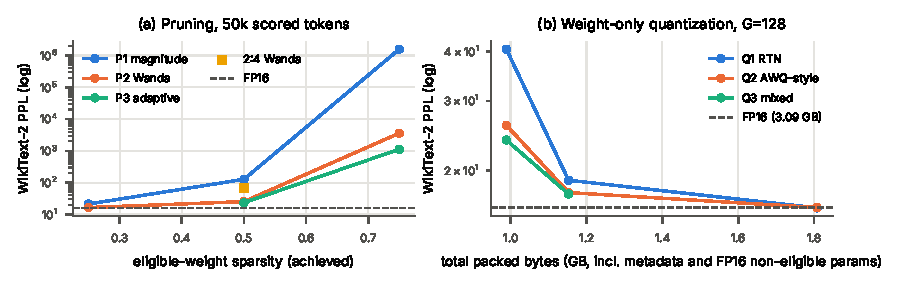
\includegraphics[width=\linewidth]{t1_tradeoff.pdf}
\caption{Held-out WikiText-2 perplexity (50{,}000 scored tokens) of Qwen2.5-1.5B versus (a) achieved sparsity and (b) total packed bytes including group metadata and uncompressed FP16 parameters. FP16 reference dashed.}
\label{fig:t1}
\end{figure}

\begin{table}[t]
\centering\footnotesize\setlength{\tabcolsep}{3.4pt}
\caption{Task 1 summary (Qwen2.5-1.5B, \GPUone). HellaSwag: zero-shot acc\_norm (lm-eval preprocessing, character-length normalisation); $n$ = 2{,}000 IDs or the first 512. $\Delta$ is the paired change versus FP16 on the same IDs (percentage points). Size = total bytes in the representation stated (FP16 dense; sparse: 1 mask bit/weight + 16 bits/nonzero; quantized: packed). All conditions run with dense FP16 kernels, so prefill latency at 2,048 tokens was \PrefillLo--\PrefillHi\,ms, decode \DecLo--\DecHi\,ms/token and peak allocated memory \PeakGB\,GB for every row.}
\label{tab:t1}
\begin{tabular}{@{}llrrrrrrr@{}}
\toprule
Condition & Budget & Wiki PPL & C4 PPL & HS (n) & $\Delta$HS & Size MB & Calib.\ err & Compr.\ s\\
\midrule
\gentab{t1_summary}
\bottomrule
\end{tabular}
\end{table}

\begin{table}[t]
\centering\footnotesize\setlength{\tabcolsep}{4pt}
\caption{Paired 95\% bootstrap intervals at matched budgets (2{,}000 resamples; PPL resamples whole evaluation windows). HellaSwag in percentage points over the IDs scored for both conditions ($n$).}
\label{tab:t1boot}
\begin{tabular}{@{}lrrr@{}}
\toprule
Comparison & $\Delta$ WikiText-2 PPL & $\Delta$ C4 PPL & $\Delta$ HellaSwag acc\_norm (pp)\\
\midrule
\gentab{t1_boot}
\bottomrule
\end{tabular}
\end{table}

\begin{figure}[t]
\centering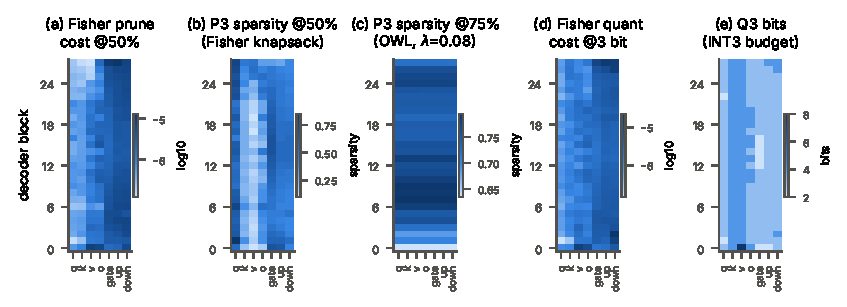
\includegraphics[width=\linewidth]{t1_maps.pdf}
\caption{Sensitivity probes (calibration data only) and final allocations over 28 blocks $\times$ 7 projections: (a) Fisher cost of Wanda-pruning 50\% of a projection; (b,c) selected P3 sparsity maps; (d) Fisher-weighted 3-bit perturbation; (e) selected Q3 bits at the INT3 budget.}
\label{fig:t1maps}
\end{figure}

\textbf{Magnitude, activation and removal impact.} Magnitude and Wanda masks overlap heavily (Jaccard \JacTwentyFive{} at 25\%, \JacSeventyFive{} at 75\%; at 50\% lowest for o\_proj, \JacO, highest for gate\_proj, \JacGate), but the differing minority decides quality: input channels reach norms of \ActMax{} (down\_proj, blocks 1--2 and 26), so small weights on outlier channels carry large outputs.
Weighting by $\|X_j\|$ cuts 50\% perplexity by 102 points, adds 17.8\,pp HellaSwag (Table~\ref{tab:t1boot}) and halves calibration layer-output error (0.064$\to$0.027, Table~\ref{tab:t1}). At 75\% every uniform method collapses (PPL $>$3{,}600, HellaSwag near chance).

\textbf{Sensitivity and allocation.} Summed per projection the MLP matrices carry the largest Fisher costs (Fig.~\ref{fig:t1maps}a,d), but per weight the small k/v projections are most sensitive, so both allocators protect them: P3 at 50\% keeps v\_proj at 21\% and k\_proj at 30\% sparsity while pruning q\_proj to 63\% (Fig.~\ref{fig:t1maps}b).
Q3 gives k/v projections 8 bits in \QfourKVeight\% of blocks at the INT4 budget (\QfourHist) and pays with 2--3-bit gate/up matrices (INT3: \QthreeHist).
At 75\% the development set preferred OWL, which protects early blocks (Fig.~\ref{fig:t1maps}c); the additive diagonal-Fisher model misses interactions once most of a layer is removed.

\textbf{Uniform versus adaptive at matched budgets.} The adaptive allocations improve likelihood significantly in all four comparisons (Table~\ref{tab:t1boot}): $-2.0$ WikiText-2 PPL at 50\% and 75\% sparsity going from 3{,}614 to 1{,}130; $-0.15$ and $-2.14$ for Q3 at the INT4 and INT3 budgets.
HellaSwag improves only at 75\% (+7.0\,pp); the other intervals include zero, since a 0.5--2 point perplexity change barely moves four-way \emph{relative} likelihoods and the 2{,}000-example CI half-width is $\approx$1\,pp. C4 gains are smaller, and the Q3 INT4 C4 interval includes zero, so evidence for Q3 at INT4 is weak.
AWQ-style scaling matters more than allocation: at INT3 it removes 14.5 PPL and adds 5.7\,pp HellaSwag over round-to-nearest.
The first 512 HellaSwag IDs are harder (FP16 \HSfirst\% vs.\ \HSrest\%), so only paired deltas on identical IDs are compared.

\textbf{Calibration criteria versus held-out quality.} Calibration layer-output error ranks held-out WikiText-2 perplexity almost perfectly (Spearman $\rho=\RhoCalWiki$) and development NLL ranks HellaSwag well ($\rho=\RhoDevHS$), so test-free dev selection was a sound proxy. A fixed qualitative case (HellaSwag ID 63, the first FP16-correct example missed by P2@50\%) is missed by all three 50\% pruners but kept by every INT3 quantizer (Appendix~\ref{app:qual}).

\textbf{Theoretical versus practical savings.} Packed INT3 is 989 vs.\ 3{,}087\,MB in FP16 (32\%; eligible weights alone shrink to 20\%, the \OtherMB\,MB embedding caps the ratio). 50\% sparsity in mask+value format saves only 37\% (1.125 vs.\ 2 bytes/weight). Latency and memory are identical across all 18 conditions because zeros and dequantized weights still run as dense FP16 GEMMs; the hardware-supported 2:4 format costs +42 PPL and $-9.8$\,pp HellaSwag versus unstructured Wanda. Compression takes 31--35\,s (pruning) or 131\,s (AWQ search), plus a one-off \ProbeS\,s probe (Fisher \FisherS\,s).

\section{Task 2: Efficient attention and context memory}\label{sec:t2}
\subsection{Exact attention}
\begin{figure}[t]
\centering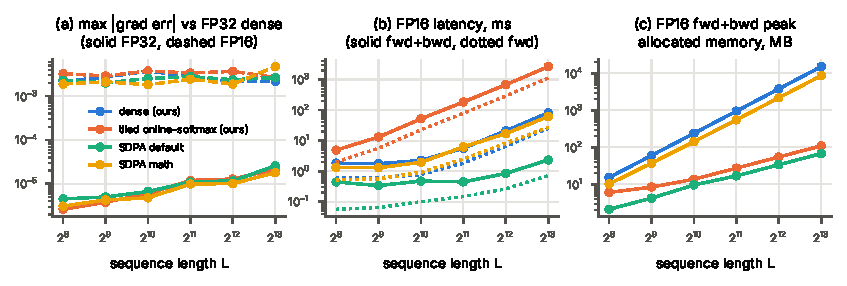
\includegraphics[width=\linewidth]{t2_attention.pdf}
\caption{Exact causal attention, $B{=}2$, $H{=}4$, $d{=}64$, \GPUtwo, 10 warmed repetitions. (a) gradient error against dense FP32; (b) FP16 latency; (c) FP16 forward+backward peak allocated memory. Our tiled kernel is a Python loop over $128\times128$ tiles with a recomputation backward that stores only $O$ and the log-sum-exp, not a fused FlashAttention kernel.}
\label{fig:t2a}
\end{figure}
\begin{table}[t]
\centering\footnotesize\setlength{\tabcolsep}{4pt}
\caption{Backends at $L{=}8{,}192$, FP16 (errors vs dense FP32). Flash and cuDNN SDPA reject FP32 inputs. Default dispatch: FP16 $\to$ \DefaultSixteen, FP32 $\to$ \DefaultThirtyTwo{} (from profiler kernel names).}
\label{tab:t2a}
\begin{tabular}{@{}lcrrrrr@{}}
\toprule
Implementation & FP32 & fwd ms & fwd+bwd ms & peak MB & max$|\Delta O|$ & max$|\Delta \nabla|$\\
\midrule
\gentab{t2_attn}
\bottomrule
\end{tabular}
\end{table}
In FP32 our tiled online-softmax attention matches dense to \TiledErrOut{} (output) and \TiledErrGrad{} (gradients) at every length and all seven tile shapes (forward memory \TileMinMB--\TileMaxMB\,MB at $L{=}1{,}024$); in FP16 all methods sit at the $\sim$$10^{-3}$ rounding floor (Fig.~\ref{fig:t2a}a), and perturbing future keys/values changes no earlier output.
With $30\times$ scaled queries, our dense FP16 kernel deviates from FP64 by \ExtremeDenseSixteen{} against \ExtremeSdpaSixteen{} for SDPA, because it forms $QK^\top$ in FP16 whereas the fused kernels accumulate in FP32.
The score matrix dominates memory: at $L{=}8{,}192$ dense forward+backward needs 15.1\,GB, SDPA math 8.6\,GB, our tiled kernel 109\,MB and fused SDPA 68\,MB. Tiling delivers the memory saving, but without fusion each of $\sim$2{,}000 tiles is a separate launch (2.65\,s vs.\ 2.3\,ms; Table~\ref{tab:t2a}).

\subsection{Associative recall (MQAR)}
\begin{figure}[t]
\centering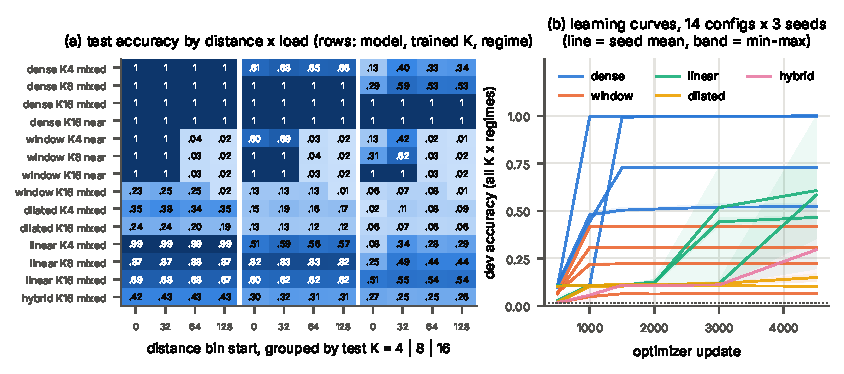
\includegraphics[width=\linewidth]{t2_mqar.pdf}
\caption{MQAR, 2-layer $d{=}128$ models (0.44M parameters, all within 0.5\%), 4{,}500 updates, 3 seeds. (a) Test accuracy by source--query distance and test-time number of pairs $K$ (1{,}024 sequences per $K\times$regime); label chance 1/64. (b) Development accuracy curves for all 14 configurations.}
\label{fig:t2b}
\end{figure}
\begin{table}[t]
\centering\scriptsize\setlength{\tabcolsep}{2.6pt}
\caption{MQAR test accuracy at the trained $K$ (mean$\pm$sd over seeds; per-seed mixed accuracy listed), theoretical attended pairs per head and decoding state (floats per layer) at $T{=}256$, and measured training cost (\GPUtwo).}
\label{tab:t2b}
\resizebox{\linewidth}{!}{\begin{tabular}{@{}lrlrrrlrrrr@{}}
\toprule
Mechanism & $K$ & Train & Near & Far & Mixed & Mixed per seed & Pairs & State & ms/step & Peak MB\\
\midrule
\gentab{t2_mqar}
\bottomrule
\end{tabular}}
\end{table}
Dense attention solves every trained setting and generalises across distance: trained on near pairs only, it reaches 1.00 on far pairs (Table~\ref{tab:t2b}).
It does not generalise across load: the $K{=}4$ model scores 0.33 on mixed $K{=}16$ queries (Fig.~\ref{fig:t2b}a).
The $W{=}64$ window answers near queries perfectly but far ones at chance (\WinFar), as its 126-position two-layer receptive field implies.
Imposing the same mask on dense models only at test time gives an identical profile (near \MaskNear, far \MaskFar), so the failure is reach, not learning; keeping each query's 64 \emph{highest-scoring} keys loses nothing (mixed \TopkMixed). Training on unreachable queries is itself harmful: window and dilated models trained on mixed data never learn, even at reachable distances (loss \WinMixLoss{} vs.\ $\ln 64=\LnSixtyFour$).
Linear attention is flat across distance but falls with load (0.99, 0.82, 0.54 for $K=4,8,16$) and is bimodal across seeds (one $K{=}16$ seed solves it; others 0.47, 0.16): its 4.2k-float state, not distance, limits it.
\textbf{B3.} The intervention was a per-head gated mix of an 8-token softmax window and a 16-feature ELU+1 memory, with the state held below the linear comparator (4{,}160 vs 4{,}224 floats) and +0.5\% parameters. Our prediction (committed before any B3 result) that it would beat linear attention at $K{=}16$ was falsified: 0.26$\pm$0.23 vs.\ 0.54$\pm$0.42. Halving the feature dimension costs more capacity than the window recovers.
\textbf{Theory versus measurement.} At $T{=}256$ the window attends to 44\% of dense pairs and linear attention keeps $O(1)$ state. In the forward-only sweep at $T{=}8{,}192$, however, the window takes \SwWindowMs\,ms and \SwWindowMB\,MB against \SwDenseMs\,ms and \SwDenseMB\,MB for dense causal SDPA. (the boolean mask forces a non-fused path); linear attention takes \SwLinearMs\,ms and \SwLinearMB\,MB (our parallel form materialises $[B,H,T,f,d]$ prefixes) and top-$k$ \SwTopkMs\,ms and \SwTopkMB\,MB.

\subsection{KV-cache compression at a matched INT4 byte budget}
\begin{table}[t]
\centering\footnotesize\setlength{\tabcolsep}{2.8pt}
\caption{Qwen2.5-1.5B-Instruct on 180 retrieval prompts (\KvLctxLo--\KvLctxHi{} context tokens), each policy at the per-prompt serialised size of the uniform INT4 channel-K/token-V cache. EM: exact match (FP16 is correct on all prompts, so conditional = unconditional). NLL of the gold code; KL(FP16$\|$policy) at the first answer token and over teacher-forced positions. Evid.: evidence tokens kept in FP16 (layer mean). Live: cache at end of decoding. Peak: allocated memory incl.\ dequantized copies.}
\label{tab:kv}
\resizebox{\linewidth}{!}{\begin{tabular}{@{}lrrrrrrrrr@{}}
\toprule
Policy & EM\% & NLL & KL$_1$ & KL$_\text{TF}$ & Evid.\% & Packed MB & \% FP16 & Live MB & Peak GB\\
\midrule
\gentab{t2_kv}
\bottomrule
\end{tabular}}
\end{table}
\begin{table}[t]
\centering\scriptsize\setlength{\tabcolsep}{3.5pt}
\caption{EM\% by factor (FP16, sink+recent, question-aware, INT4 token-wise, INT4 channel-K, hybrid; columns as Table~\ref{tab:kv}).}
\label{tab:kvb}
\begin{tabular}{@{}lrrrrrrr@{}}
\toprule
Factor & $n$ & FP16 & S+R & QA & Tok & Chan & Hyb\\
\midrule
\gentab{t2_kvbreak}
\bottomrule
\end{tabular}
\end{table}
\begin{table}[t]
\centering\scriptsize\setlength{\tabcolsep}{4pt}
\caption{C5: real bit packing at 5{,}217 context tokens, 10 repetitions (\GPUtwo; 2{,}633 tokens in Appendix~\ref{app:supp}). Serialised bytes match the handout formula exactly. Size, decode step (including unpacking) and peak allocated memory: packed / FP16.}
\label{tab:c5}
\begin{tabular}{@{}rrlrrrrr@{}}
\toprule
Ctx tokens & Batch & Layout & MB & pack ms & unpack ms & step ms & peak GB\\
\midrule
\gentab{t2_c5_main}
\bottomrule
\end{tabular}
\end{table}
All C1 checks pass: the rebuilt full-retention cache reproduces ordinary greedy generation on 180/180 prompts, and split prefill differs from a single forward by at most \KvSplit{} in FP16 logits.
At the matched budget (28.7\% of FP16 bytes; \KvEvictN{} of $\sim$3{,}900 positions kept by eviction), question-aware eviction, channel-wise-key INT4 and the hybrid all retrieve essentially perfectly (Table~\ref{tab:kv}). Question-aware eviction beats sink+recent by \KvQaSink\,pp.
Sink+recent succeeds only when evidence is recent (Table~\ref{tab:kvb}) and never abstains: of \SinkWrong{} failures, \SinkInCtx{} give another in-context code, the rest invent one. The question-aware scorer keeps \QaEvLzero\% of evidence in layer~0 and \QaEvLtwo\% from layer~2 on.
Grouping decides the quantized results. Token-wise INT4 shares each 64-feature group with Qwen's key outlier channels, which inflates relative key error from \KvKmseKivi{} to \KvKmseTok{} (values identical at \KvVmse). The model then degenerates into repetition (``river river \dots'') on every prompt.
Exact match saturates, so likelihood separates the three good policies: gold-code NLL relative to question-aware eviction is \KvNllKiviQa{} for channel INT4 and \KvNllHybQa{} for the hybrid, whose INT2 values (relative error \KvVmseHyb) cost one middle-position failure.
\textbf{Systems.} Prefill takes \KvPrefill\,ms, question scoring an extra \KvScoring\,ms, and eviction after full prefill leaves the prefill peak (\KvPrefillPeak\,GB) unchanged. Packing (Table~\ref{tab:c5}) stores exactly the formula's bytes, but SDPA needs FP16, so each decode step unpacks ($\sim$12\,ms at batch~1; step 34$\to$46--49\,ms) and peak memory is \emph{higher} than FP16 because both copies coexist.

\section{Task 3: Draft distillation and exact speculative decoding}\label{sec:t3}
\textbf{Sampler correctness.} The sampler~\cite{leviathan,chen2023} verifies all $\gamma$ proposals in one target pass, samples corrections from $\mathrm{norm}([p-q]_+)$, adds a bonus token after full acceptance, stops at EOS and crops both KV caches.
On 100{,}000 length-3 sequences of a 3-symbol Markov target ($\gamma{=}2$) the empirical law matches the exact one ($\chi^2=\ChiStat$, 26 dof, $p=\ChiP$); replacing the residual by $p$ is rejected ($\chi^2=\ChiNeg$); EOS ($p=\ChiEos$) and $\gamma{=}1$ ($p=\ChiGone$) variants pass.
On the real models, cached and recomputed next-token distributions agree to \CacheDiff{} after rollbacks, and the 120-prompt exact-speculative prefix bank matches the target's own samples: paired $\Delta\mathbb{E}[1-\mathrm{TV}]=$ \ConsDiff; mean target log-probability of sampled tokens \ConsLogpS{} vs.\ \ConsLogpT.
\textbf{Distillation.} LoRA~\cite{lora} ($r{=}8$ on q/k/v/o, \AdapterParams{} parameters, 0.22\% of \StudentParams) is trained on forward token-level KL from the frozen \TeacherParams{} teacher~\cite{distillspec,gkd}. Each run used exactly 30{,}000 GSM8K + 10{,}000 short-form teacher-scored tokens, 157 updates and one skipped FP16-overflow step.
Off-policy runs take 56\,min, dominated by the shared 800-response teacher pool (52.6\,min; \PoolLen{} responses hit the 192-token cap); on-policy runs take 36\,min, dominated by student rollouts (32.6\,min); scoring and training take $<$4\,min, merging changes logits by $\le$0.41 and peak memory is 5.3\,GB (Table~\ref{tab:t3d}, appendix). Training KL (Fig.~\ref{fig:t3}a) is measured on each method's own prefixes, so it is not comparable across methods.


\begin{table}[t]
\centering\scriptsize\setlength{\tabcolsep}{4pt}
\caption{Standalone accuracy (\%, greedy decoding; 512/32-token caps). Short form: exact match / answer present.}
\label{tab:t3s}
\begin{tabular}{@{}lrrrr@{}}
\toprule
Model & GSM8K acc. & GSM8K truncated & Familiar & Shifted\\
\midrule
\gentab{t3_standalone}
\bottomrule
\end{tabular}
\end{table}

\begin{figure}[t]
\centering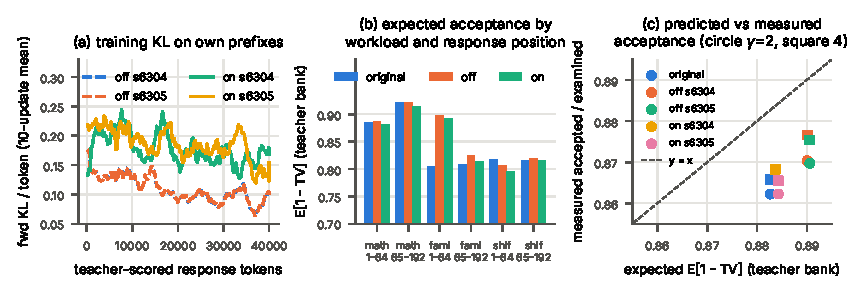
\includegraphics[width=\linewidth]{t3_distill_align.pdf}
\caption{(a) Distillation KL per teacher-scored token. (b) Expected one-token acceptance on the teacher prefix bank by workload and response position (seed means). (c) Bank-predicted versus measured acceptance in speculative decoding ($n{=}240$ requests per point).}
\label{fig:t3}
\end{figure}

\begin{table}[t]
\centering\footnotesize\setlength{\tabcolsep}{3pt}
\caption{Common-prefix alignment of drafts with the 1.5B target: forward KL, reverse KL and $\mathbb{E}[1-\mathrm{TV}]$ (number of positions; trained-draft entries are seed means $\pm$ sd over the two seeds).}
\label{tab:t3a}
\resizebox{\linewidth}{!}{\begin{tabular}{@{}l rrr rrr rrr@{}}
\toprule
& \multicolumn{3}{c}{Original 0.5B} & \multicolumn{3}{c}{Off-policy} & \multicolumn{3}{c}{On-policy}\\
\cmidrule(lr){2-4}\cmidrule(lr){5-7}\cmidrule(lr){8-10}
Prefix bank & fKL & rKL & E[acc] & fKL & rKL & E[acc] & fKL & rKL & E[acc]\\
\midrule
\gentab{t3_align}
\bottomrule
\end{tabular}}
\end{table}

\begin{table}[t]
\centering\scriptsize\setlength{\tabcolsep}{2.2pt}
\caption{Speculative decoding, 120 prompts $\times$ 2 counterbalanced repetitions, EOS-aware 64-token cap, temperature 1, \GPUthree. Times: ms/request (draft / verify / accept+rollback / prefill). tok/s: speculative / adjacent target-only. Decode speedup: target over speculative decode time per output token [paired 95\% CI]. $c$, $v_\gamma$: measured costs relative to a target step; $\hat S$: predicted speedup; $\alpha^*$: break-even acceptance. ``Fixed 64'' ignores EOS (timing only).}
\label{tab:t3spec}
\resizebox{\linewidth}{!}{\begin{tabular}{@{}lrrrrrrlrlrrrr@{}}
\toprule
Draft & $\gamma$ & acc/exam & acc/prop & prefix & tgt/tok & drf/tok & time decomposition & tok/s & decode speedup & $c$ & $v_\gamma$ & $\hat S$ & $\alpha^*$\\
\midrule
\gentab{t3_spec}
\bottomrule
\end{tabular}}
\end{table}

\textbf{Alignment.} Distillation lowers forward KL on every common bank, e.g.\ from 0.174 to 0.146 (off) and 0.150 (on) on teacher samples, but raises expected acceptance by at most 0.01 (Table~\ref{tab:t3a}).
The gain is concentrated where training data resembled the evaluation: on familiar short-form templates, early-position acceptance rises from \FamExpOrig{} to \FamExpOff, whereas math is unchanged and shifted templates do not improve (Fig.~\ref{fig:t3}b). The improvement does not transfer to unseen formats.
On-policy drafts have lower forward KL on student rollouts but no higher acceptance; seed variation is $\le$0.001. The largest decoded disagreement is the first token: the original draft opens familiar answers with ``To'' where the target says ``The'' (TV 0.73--0.75), which distillation fixes (TV $\le$0.09).
\textbf{Speculative execution.} Acceptance is high (0.86--0.88 of examined proposals, 1.6/2.7 accepted per round at $\gamma=2/4$), and target passes fall to 0.39/0.27 per output token. Yet every configuration is slower than target-only decoding: decode speedup is 0.80--0.83 with all intervals below 1 (Table~\ref{tab:t3spec}).
A 0.5B draft step takes \StepDraft\,ms against \StepTarget\,ms for the target (verifying 5 tokens: \StepVerifyFive\,ms): batch-1 eager decoding is launch-bound and scales with layer count (24 vs.\ 28), not parameters, so $c\approx0.86$--$0.90$, $v_\gamma\approx1.2$, $\hat S=0.82$--$0.88$ and break-even needs $\alpha^*\ge0.96$. Measured ratios (0.78--0.81) sit 0.03--0.06 below $\hat S$ (host overhead); drafting takes 54--70\% of request time, verification 26--38\%, rollback $<$1\%. Bank-predicted acceptance ranks drafts correctly but overestimates by 1--2 points (Fig.~\ref{fig:t3}c).
Distilled drafts improve throughput over the original by +0.010 to +0.014 at $\gamma{=}2$ (\PairOffOrig), with no significant gain at $\gamma{=}4$. On- and off-policy drafts are indistinguishable in every paired comparison (acceptance differences \OnOffRange; \OnOffAllZero{} intervals include 0).
\textbf{Workload and cost.} Acceptance is lowest on shifted templates (\ShAccOff{} vs.\ \MathAccOff{} for math); ignoring EOS (fixed 64) raises speedup only to 0.87--0.88, and an unmerged adapter gives $c=1.27$ (speedup 0.56).
Standalone, distillation fixes knowledge but not format: every familiar answer is present in the distilled students' replies (vs.\ 67\% for the original draft), yet strict exact match stays at 33\% for all models, teacher included (Table~\ref{tab:t3s}).
Because no draft beats target-only decoding, distillation cannot pay for itself here. Against the original draft only off-s6304 at $\gamma{=}4$ saves time (\BeSave\,ms per request), which would take $\sim$\BeReq{} requests to recover its \BeCost-minute cost.

\FloatBarrier
\section{Conclusion}
Nominal efficiency ratios proved reliable predictors of storage and of algorithmic correctness, but poor predictors of measured speed and memory. Compressed weights still execute as dense FP16, tiled attention saves memory but not time without fusion, packed KV caches must be unpacked, and a small draft is not cheap when decoding is launch-bound.
Within each comparison, information-aware choices consistently beat position- or magnitude-only ones: activation-aware masks, content-selected attention, question-aware eviction and channel-wise key grouping.
Adaptive allocation and on-policy distillation gave small or statistically indistinguishable gains at matched budgets, and we report them as such.

\small
\begin{thebibliography}{99}
\bibitem{qwen25} Qwen Team. Qwen2.5 technical report. \emph{arXiv:2412.15115}, 2024.
\bibitem{pytorch} A.~Paszke et al. PyTorch: An imperative style, high-performance deep learning library. In \emph{NeurIPS}, 2019.
\bibitem{hf} T.~Wolf et al. Transformers: State-of-the-art natural language processing. In \emph{EMNLP: System Demonstrations}, 2020.
\bibitem{c4} C.~Raffel et al. Exploring the limits of transfer learning with a unified text-to-text transformer. \emph{JMLR}, 21(140), 2020.
\bibitem{wikitext} S.~Merity, C.~Xiong, J.~Bradbury, R.~Socher. Pointer sentinel mixture models. In \emph{ICLR}, 2017.
\bibitem{hellaswag} R.~Zellers, A.~Holtzman, Y.~Bisk, A.~Farhadi, Y.~Choi. HellaSwag: Can a machine really finish your sentence? In \emph{ACL}, 2019.
\bibitem{gsm8k} K.~Cobbe et al. Training verifiers to solve math word problems. \emph{arXiv:2110.14168}, 2021.
\bibitem{lmeval} L.~Gao et al. A framework for few-shot language model evaluation (lm-evaluation-harness). Zenodo, 2023.
\bibitem{wanda} M.~Sun, Z.~Liu, A.~Bair, J.~Z.~Kolter. A simple and effective pruning approach for large language models. In \emph{ICLR}, 2024.
\bibitem{obd} Y.~LeCun, J.~S.~Denker, S.~A.~Solla. Optimal brain damage. In \emph{NeurIPS}, 1990.
\bibitem{molchanov} P.~Molchanov, A.~Mallya, S.~Tyree, I.~Frosio, J.~Kautz. Importance estimation for neural network pruning. In \emph{CVPR}, 2019.
\bibitem{owl} L.~Yin et al. Outlier weighed layerwise sparsity (OWL): A missing secret sauce for pruning LLMs to high sparsity. In \emph{ICML}, 2024.
\bibitem{awq} J.~Lin et al. AWQ: Activation-aware weight quantization for on-device LLM compression and acceleration. In \emph{MLSys}, 2024.
\bibitem{hawq} Z.~Dong et al. HAWQ-V2: Hessian aware trace-weighted quantization of neural networks. In \emph{NeurIPS}, 2020.
\bibitem{flash} T.~Dao, D.~Y.~Fu, S.~Ermon, A.~Rudra, C.~R\'e. FlashAttention: Fast and memory-efficient exact attention with IO-awareness. In \emph{NeurIPS}, 2022.
\bibitem{flash2} T.~Dao. FlashAttention-2: Faster attention with better parallelism and work partitioning. In \emph{ICLR}, 2024.
\bibitem{longformer} I.~Beltagy, M.~E.~Peters, A.~Cohan. Longformer: The long-document transformer. \emph{arXiv:2004.05150}, 2020.
\bibitem{linear} A.~Katharopoulos, A.~Vyas, N.~Pappas, F.~Fleuret. Transformers are RNNs: Fast autoregressive transformers with linear attention. In \emph{ICML}, 2020.
\bibitem{zoology} S.~Arora et al. Zoology: Measuring and improving recall in efficient language models. In \emph{ICLR}, 2024.
\bibitem{based} S.~Arora et al. Simple linear attention language models balance the recall-throughput tradeoff. In \emph{ICML}, 2024.
\bibitem{streaming} G.~Xiao, Y.~Tian, B.~Chen, S.~Han, M.~Lewis. Efficient streaming language models with attention sinks. In \emph{ICLR}, 2024.
\bibitem{snapkv} Y.~Li et al. SnapKV: LLM knows what you are looking for before generation. In \emph{NeurIPS}, 2024.
\bibitem{kivi} Z.~Liu et al. KIVI: A tuning-free asymmetric 2bit quantization for KV cache. In \emph{ICML}, 2024.
\bibitem{leviathan} Y.~Leviathan, M.~Kalman, Y.~Matias. Fast inference from transformers via speculative decoding. In \emph{ICML}, 2023.
\bibitem{chen2023} C.~Chen et al. Accelerating large language model decoding with speculative sampling. \emph{arXiv:2302.01318}, 2023.
\bibitem{distillspec} Y.~Zhou et al. DistillSpec: Improving speculative decoding via knowledge distillation. In \emph{ICLR}, 2024.
\bibitem{gkd} R.~Agarwal et al. On-policy distillation of language models: Learning from self-generated mistakes. In \emph{ICLR}, 2024.
\bibitem{lora} E.~J.~Hu et al. LoRA: Low-rank adaptation of large language models. In \emph{ICLR}, 2022.
\bibitem{peft} S.~Mangrulkar et al. PEFT: State-of-the-art parameter-efficient fine-tuning methods. GitHub, 2022.
\bibitem{efron} B.~Efron, R.~J.~Tibshirani. \emph{An Introduction to the Bootstrap}. Chapman \& Hall, 1993.
\end{thebibliography}
\normalsize

\appendix
\section{Implementation details, constraints and deviations}\label{app:impl}
\textbf{Reuse and tools.} No external source files were copied. Wanda, AWQ's pseudo-quantizer conventions, OWL, the lm-eval HellaSwag preprocessing~\cite{lmeval} and the FlashAttention-2 recurrences~\cite{flash,flash2} were re-implemented from their papers and reference code. RoPE/GQA helpers come from Transformers~\cite{hf} and LoRA from PEFT~\cite{peft}. The question-aware KV scorer is a simplified fixed policy inspired by SnapKV~\cite{snapkv} (per-layer selection shared by both KV heads, attention mass of the question suffix, average pooling of width 7), with 8 sink and 64 recent safeguards~\cite{streaming}; it is not the published head-specific algorithm. Channel-K/token-V grouping follows KIVI~\cite{kivi}; the dilated and linear mechanisms follow~\cite{longformer,linear,zoology,based}.
\textbf{Course-script deviation.} The course \texttt{setup\_data.py --prefix-banks} fails under the pinned \texttt{transformers==4.57.1} because \texttt{generate()} rejects a \texttt{generator} argument. \texttt{scripts/make\_prefix\_banks.py} reproduces its prompts, seeds, positions, format and path with a seeded ancestral sampler.
\textbf{Constraints.} Flash/cuDNN SDPA do not accept FP32. Masked mechanisms use dense boolean masks (correctness implementations, not sparse kernels). KV quantization stores dequantized values for SDPA. Speculative and target-only timings run with both models resident, so their peak memory (4.19\,GB) is identical by construction. 54\% of speculative requests reach the 64-token cap (math always does), so speed-test outputs are never scored as solutions; answer accuracy uses separate 512-token greedy runs. Because speculative and target-only outputs are independent samples of different lengths, per-request throughput ratios in output-length bins are confounded, so we report the decode-time-per-token ratio. The first WikiText-2 windows are section headings, so the planned model-continuation probe produced empty continuations; qualitative analysis therefore uses HellaSwag cases.
\textbf{Resumability.} All runs checkpoint to Google Drive with atomic writes. One distillation run resumed from a checkpoint and is verified identical to an uninterrupted run by a unit test.
\textbf{AI assistance.} An LLM coding assistant (Claude) was used to help write and test the code and to draft text, as permitted by the course policy. \textit{[Edit to match your actual use.]}

\section{Qualitative cases}\label{app:qual}
\textbf{HellaSwag (Task 1).} The IDs are fixed in advance: the first four diagnostic IDs and the first four where FP16 is correct and P2@50\% is wrong. Candidate log-likelihoods for every condition are in \texttt{results/task1/qualitative.json}. On ID 63 (``He moves closer to the camera\dots''; gold ending 2), FP16 and all three INT3 quantizers choose ending 2, while P1, P2 and P3 at 50\% all switch to ending 0. On ID 16 every compressed model, quantized or pruned, switches away from the gold ending.
\textbf{KV (Task 2).} Six fixed prompts (first ID of each length$\times$position cell with 8 distractors). In \texttt{KV-2048-middle-8-00} the evidence ``access code \dots{} is 84561'' is recovered by FP16, question-aware eviction, both channel-wise caches and the hybrid. Sink+recent, which discarded the span, answers 20488. Token-wise INT4 outputs no code. Selection masks for layers 0, 14 and 27 are in \texttt{results/task2/kv/aligned.json}.
\textbf{Speculative decoding (Task 3).} Matched continuations for the first math, familiar and shifted IDs are in \texttt{results/task3/spec/continuations.json}, and decoded prefix disagreements in \texttt{results/task3/align/aligned\_disagreements.json}.

\section{Supplementary results}\label{app:supp}
\begin{table}[h]
\centering\footnotesize\setlength{\tabcolsep}{3pt}
\caption{Distillation costs (minutes, \GPUthree). Updates (skipped); logit error: merged vs unmerged FP16 student.}
\label{tab:t3d}
\begin{tabular}{@{}lrrrrrrrrr@{}}
\toprule
Run & Updates & Pool & Rollouts & Scoring & Train & Merge s & Total & Logit err. & Peak GB\\
\midrule
\gentab{t3_distill}
\bottomrule
\end{tabular}
\end{table}
\begin{table}[h]
\centering\footnotesize\setlength{\tabcolsep}{4pt}
\caption{C5 packing at both context lengths (complement to Table~\ref{tab:c5}); columns as there.}
\label{tab:c5full}
\begin{tabular}{@{}rrlrrrrr@{}}
\toprule
Ctx tokens & Batch & Layout & MB & pack ms & unpack ms & step ms & peak GB\\
\midrule
\gentab{t2_c5}
\bottomrule
\end{tabular}
\end{table}

Complete numerical grids: \texttt{results/tables/*.csv} (e.g.\ \texttt{task1\_all\_conditions}, \texttt{task2b\_mqar\_per\_seed}, \texttt{task2c\_kv\_cells}, \texttt{task3\_spec\_workload}, \texttt{task3\_spec\_paired\_comparisons}). Per-condition and per-example records are in \texttt{results/task*/}.
\begin{figure}[h]
\centering
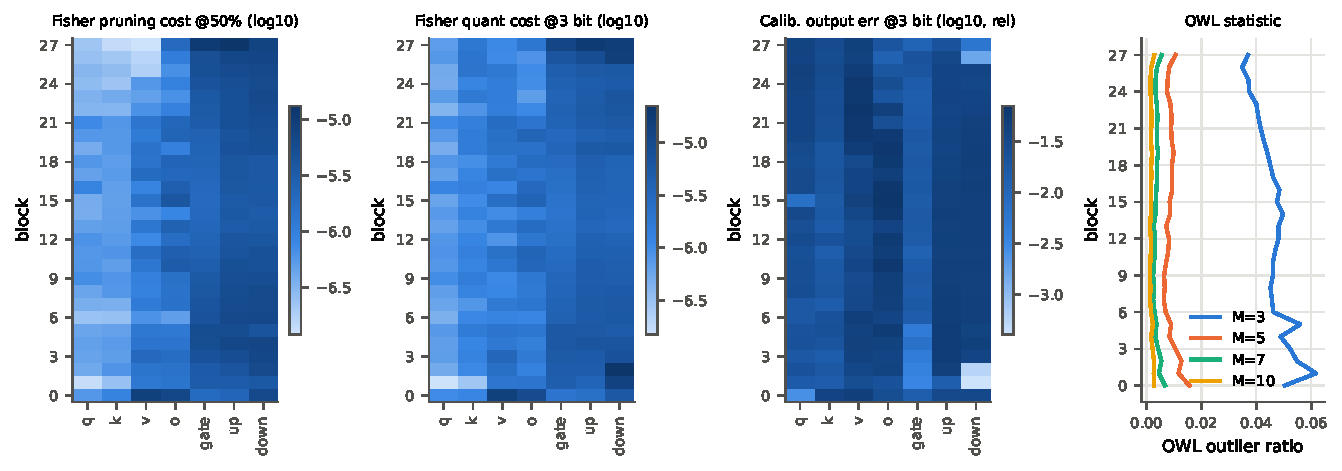
\includegraphics[width=\linewidth]{task1/sensitivity_maps.pdf}\\
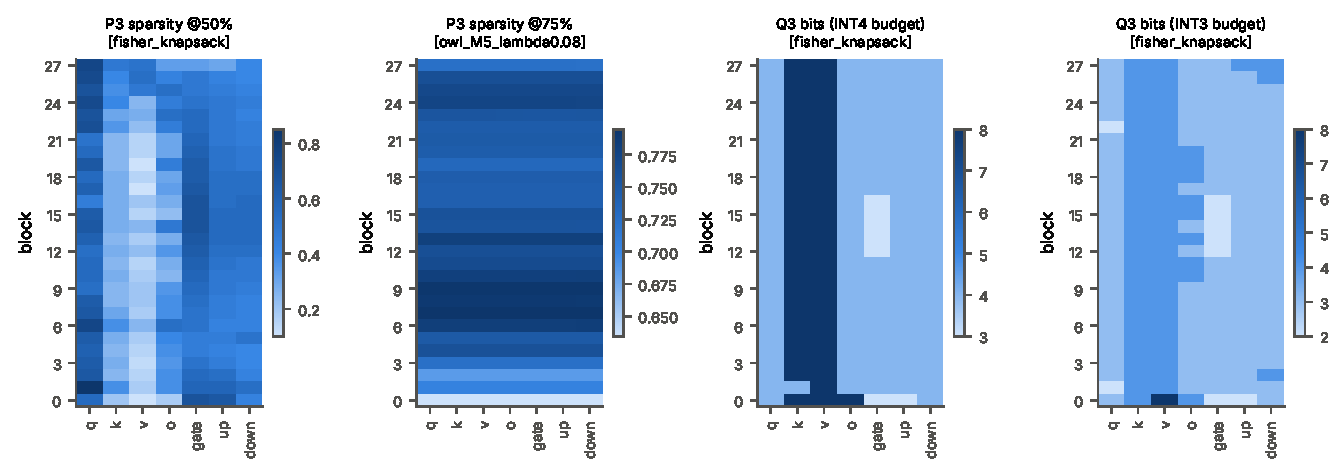
\includegraphics[width=\linewidth]{task1/allocation_maps.pdf}
\caption{All Task 1 sensitivity probes (incl.\ calibration-output error and the OWL outlier statistic for $M\in\{3,5,7,10\}$) and all four selected allocations.}
\end{figure}
\begin{figure}[h]
\centering
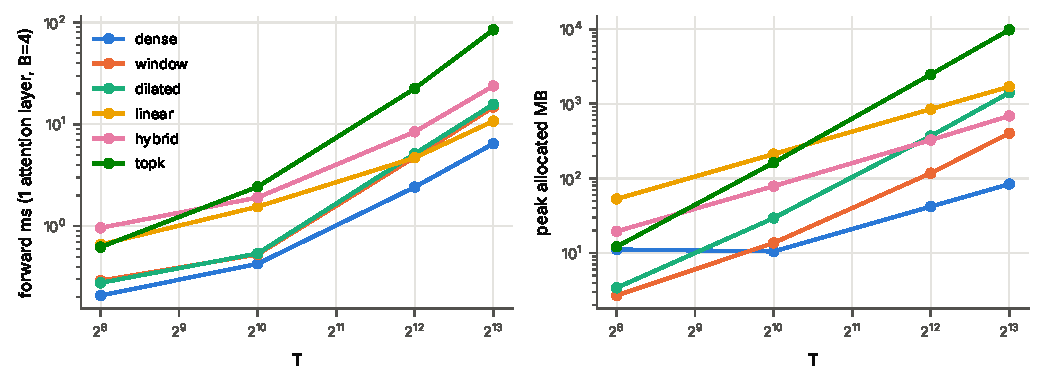
\includegraphics[width=0.49\linewidth]{task2/mqar_inference_sweep.pdf}\hfill
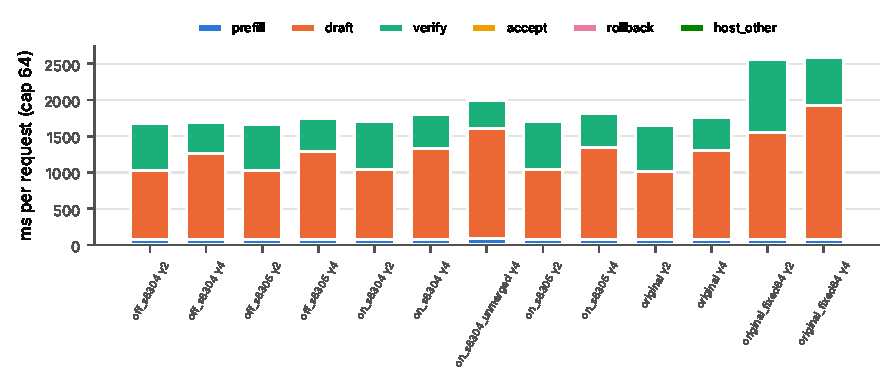
\includegraphics[width=0.49\linewidth]{task3/spec_time_decomposition.pdf}
\caption{Left: forward-only attention-layer sweep, $T\in\{256,\dots,8192\}$. Right: per-request time decomposition for every draft and $\gamma$.}
\end{figure}
\end{document}
